\chapter{Une méthode de composition dynamique des services Web
  sémantiques utilisant Neo4j}
\label{ch:approach}

\section*{Introduction}
\addcontentsline{toc}{section}{Introduction} \markboth{INTRODUCTION}{}

\newpage
\section{Reformulation du problème}
\label{sec:ch3/reformulation}

Cette section a pur but d'introduire les formalismes et les
terminologies nécessaires pour représenter et raisonner sur les
services Web. Ensuite, Nous présentons une modélisation du problème de
composition des servies Web sous forme d'un problème de recherche du
plus court chemin dans un graphe orienté.\bigskip

Chaque service web peut contenir les définitions de différentes
opérations \acrshort{wsdl} identifiables par leurs noms et leurs
paramètres. Pour des raisons de simplicité, nous supposons que chaque
service Web représente une seule opération.\medskip

\begin{mydef}[\textbf{Service Web}]
  Un Service Web $S$ est un 2-tuple $\mathpzc{<I,O>}$, où
  $\mathpzc{I}=\{I_0, \dots, I_n\}$ désigne l'ensemble des paramètres
  d'entrée, $\mathpzc{O}=\{O_0, \dots, O_m\}$ l'ensemble des
  paramètres de sortie.
\end{mydef}

%!TEX root = ../../main.tex
\begin{figure}[h]
    \centering
    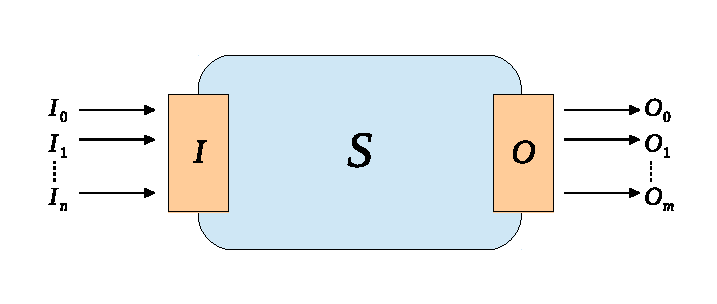
\includegraphics[width=0.65\textwidth]{figs/ch3/ws.eps}
    \caption{Un service Web atomique.}
    \label{fig:ch3/ws}
\end{figure}
%%% Local Variables:
%%% mode: latex
%%% TeX-master: "../../main"
%%% End:


Dans notre approche proposée, nous supposons que chaque service est
décrit par un document \acrshort{owls} qui possède un seule processus
atomique, et que chaque paramètre est annoté par un concept de
l'ontologie du domaine.\medskip

\begin{mydef}[\textbf{Annuaire des services Web}]
  Un annuaire des services Web est un ensemble
  $\mathpzc{R} =\{\mathit{S_0}, \mathpzc{S_1}, \dots,\mathit{S_n}\}$
  des services Web disponibles, où chaque
  $\mathpzc{S} \in \mathpzc{R}$ est un service Web décrit par un
  document \acrshort{owls}.
\end{mydef}

Afin de trouver un service composite exécutable à partir d'un annuaire
de services Web, un utilisateur doit fournir une requête de
composition.\medskip

\begin{mydef}[\textbf{Requête}]\label{def:ch3/request}
  Une requête $\mathpzc{Q}$ est un 2-tuple $\mathpzc{<I_Q, O_Q>}$.
  $\mathpzc{I_Q}$ désigne la liste des paramètres d'entrée disponibles
  (fournit par l'utilisateur ou par un autre service client), et
  $\mathpzc{O_Q}$ la listes des paramètres de sortie requis
  (objectif).
\end{mydef}

Afin de découvrir et sélectionner un service Web composite suite à une
requête de composition $\mathpzc{Q}$, les services référencés dans un
annuaire doivent être structurés dans un graphe orienté modélisant
toutes les relations de dépendance fonctionnelle possibles entre les
services disponibles deux à deux.\medskip

%!TEX root = ../../main.tex
\begin{figure}[h]
    \centering
    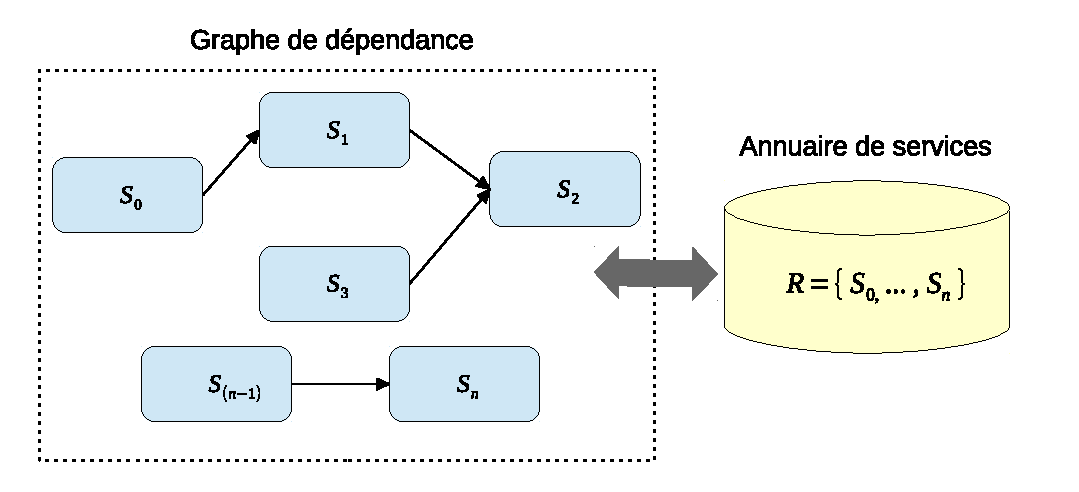
\includegraphics[width=1.1\textwidth]{figs/ch3/gd.eps}
    \caption{Graphe de dépendance $\mathpzc{GD}$ entre les services
      Web d'un annuaire $\mathpzc{R}$.}
    \label{fig:ch4/gd}
\end{figure}
%%% Local Variables:
%%% mode: latex
%%% TeX-master: "../../main"
%%% End:


\begin{mydef}[\textbf{Graphe de dépendance}]
  Un graphe de dépendance $\mathpzc{DG}$ est un ``graphe acyclique
  orienté'' $\mathpzc{DG}=<\mathpzc{R}, \mathpzc{L}>$ qui modélise
  toutes les relations de dépendance fonctionnelle possibles entre les
  services Web disponibles dans un annuaire $\mathpzc{R}$. Il existe
  une relation
  $\mathit{L_{ij}}=(\mathit{S_i}, \mathit{S_j}) \in \mathpzc{L}$ si et
  seulement s'il existe une relation de dépendance fonctionnelle entre
  $\mathit{S_i}$ et $\mathit{S_j}$, où
  $\{\mathit{S_i, S_j}\} \subset \mathpzc{R}$.\medskip
\end{mydef}

L'approche proposée consiste à construire un graphe de dépendance à
priori (\textit{Offline}) et le sauvegarder dans une base de données
graphe (\textit{Neo4j}). Suite à une requête $\mathpzc{Q}$, un
sous-graphe $\mathpzc{G}$ est extrait, qui correspond à un plan de
composition exécutable $\mathpzc{P}$ d'un service Web composite
satisfaisant.\medskip

%!TEX root = ../../main.tex
\begin{figure}[h]
    \centering
    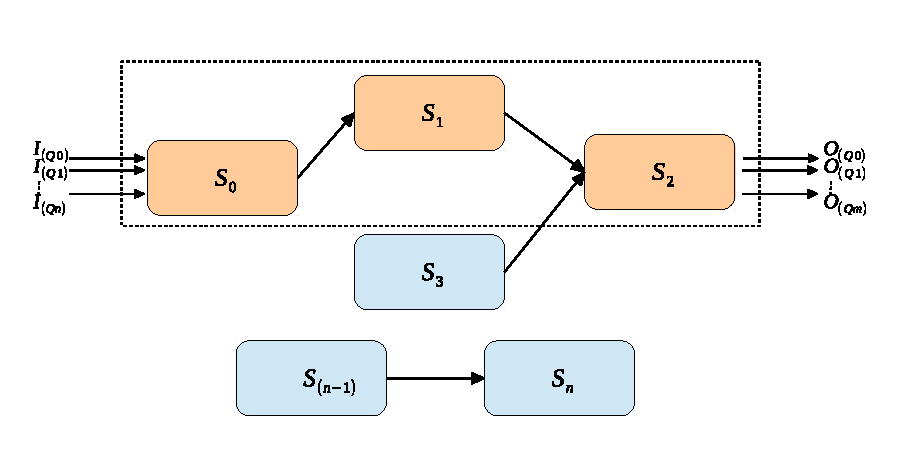
\includegraphics[width=1\textwidth]{figs/ch3/composition-plan.eps}
    \caption{Un service Web composite avec le plan de composition correspond.}
    \label{fig:ch3/composition-plan}
\end{figure}
%%% Local Variables:
%%% mode: latex
%%% TeX-master: "../../main"
%%% End:


\begin{mydef}[\textbf{Plan de composition}]
  Un plan de composition $\mathpzc{P}$ est un sous-graphe
  $\mathpzc{G \subset DG}$ d'un graphe de dépendance $\mathpzc{DG}$,
  tel que $\mathpzc{G=(R_Q,L_Q)}$ décrit le flux de données/contrôles
  d'exécution d'un ensemble de services Web atomiques
  $\mathpzc{R_Q \subset R}$ engagés dans un processus de
  composition. Il existe un lien de dépendance fonctionnelle
  (\textit{Link}) $\mathit{L_{Q_{ij}}} \in \mathpzc{L_Q}$ tel que
  $\mathit{L_{Q_{ij}}} = (S_i, S_j)$ si l'exécution d'un service
  $\mathit{S_j}$ dépend d'un ou plusieurs paramètres de sortie du
  $\mathit{S_i}$.\medskip
\end{mydef}

\begin{mydef}[\textbf{Service Web composite}]
  Un service Web composite $\mathpzc{S_Q}$ est un service Web
  exécutable composé de $n \geq 1$ services atomiques
  $\mathit{S_{0 \leq i \leq n}} \in \mathpzc{R_Q}$ tel que l'exécution
  d'un tel service correspond à l'exécution d'un plan de composition
  $\mathpzc{P}$ décrit par un graphe de dépendance
  $\mathpzc{G = <R_Q,L_Q>}$ suite à une requête $\mathpzc{Q}$.\medskip
\end{mydef}

La figure \ref{fig:ch3/composition-plan} montre un service Web
$\mathpzc{S_Q} = <\mathit{\{I_0, \dots, I_n\}}, \mathit{\{O_0, \dots,
  O_m\}}>$
correspondant à un plan de composition $\mathpzc{P}$ représenté par un
graphe de dépendances $\mathpzc{G =<R_Q,L_Q>}$, tel que
$\mathpzc{R_Q = \{S_0, S_1, S_2\}}$ et
$\mathpzc{L_Q = \{(S_0, S_1), (S_1, S_2)\}}$.\medskip

Une service Web composite $\mathpzc{S_Q = <I_S, O_S>}$ est créer et
exécuter suite à une requête de composition $\mathpzc{Q=<I_Q, O_Q>}$.
Deux conditions nécessaires et suffisantes pour que $\mathpzc{S_Q}$
satisfasse $\mathpzc{Q}$:\medskip

\begin{enumerateRoman}
\item L'interface d'entrée $\mathpzc{I_S}$ est équivalent, ou inclus
  dans $\mathpzc{I_Q}$ ($\mathpzc{I_S \subseteq I_Q}$).

\item L'interface de sortie $\mathpzc{O_Q}$ est équivalent, ou inclus
  par $\mathpzc{O_S}$ ($\mathpzc{O_Q \subseteq O_S}$).\medskip
\end{enumerateRoman}
\enddescription

Cette relation d'\emph{équivalence/inclusion} fonctionnelle entre les
interfaces d'\emph{entrée/sortie} sera abordée en détaille dans la
sections~\ref{sec:ch3/matching}.\medskip

\begin{mydef}[\textbf{Problème de composition}]
  Étant donné $\mathpzc{R}$ un annuaire des services Web et
  $\mathpzc{Q}$ une requête, Le problème de composition
  $\mathpzc{WCP=<R,Q>}$ consiste à trouver un plan optimal et
  exécutable de composition $\mathpzc{P}$ associé au service Web
  composite $\mathpzc{S_Q}$ satisfaisant la requête
  $\mathpzc{Q}$.\medskip
\end{mydef}

%!TEX root = ../../main.tex
\begin{figure}[h]
    \centering
    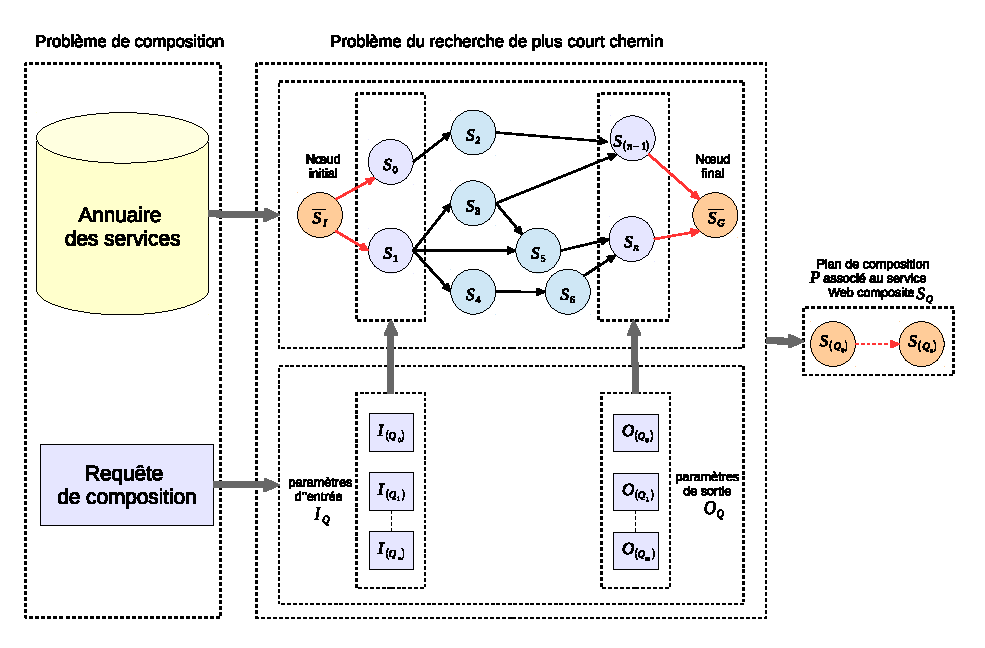
\includegraphics[width=1.15\textwidth]{figs/ch3/reformulation.eps}
    \caption{Reformulation du problème.}
    \label{fig:ch3/reformulation}
\end{figure}
%%% Local Variables:
%%% mode: latex
%%% TeX-master: "../../main"
%%% End:


La solution proposée dans ce chapitre s'appuie sur une transformation
du problème de composition défini précédemment
$\mathpzc{WCS \equiv <R,Q>}$ vers un problème du \textit{``plus court
  chemin dans un graphe orienté''}. Étant donné un graphe acyclique et
orienté $\mathpzc{DG}$, on souhaite de trouver le plus court chemin
entre un ensemble de nœuds initiales $\mathpzc{R_I \subset R}$ qui
représentent l'ensemble de services du départ, et l'ensemble de nœuds
terminaux $\mathpzc{R_O \subset R}$ qui représentent les services
d'arrivée, tel que $\mathpzc{I_S \subseteq Inputs(R_I) \subseteq I_Q}$
et $\mathpzc{O_Q \subseteq Outputs(R_O) \subseteq O_S}$.\medskip

La solution du notre problème sera donc le sous-graphe $\mathpzc{G}$
qui correspond à un plan de composition $\mathpzc{P}$. L'existence
d'une solution $\mathpzc{G}$ implique l'existence d'un service Web
composite $\mathpzc{S_Q= <R_Q, L_Q>}$, tel que
$\mathpzc{R_Q= <S_{Q_1}, \dots, S_{Q_n}>}$ et
$\mathpzc{\exists (S_{Q_i},S_{Q_j}) \in R_Q^2 \colon (S_{Q_i},S_{Q_j})
  \in (R_I \times R_O)}$.\medskip

La figure~\ref{fig:ch3/reformulation} illustre graphiquement le
processus du reformulation. Les techniques et les algorithmes du
construction des graphes $\mathpzc{DG}$ et $\mathpzc{G}$, ainsi que
leurs structures et caractéristiques, seront présentés dans les
sections~\ref{sec:ch3/graph} et~\ref{sec:ch3/composition}.\medskip

\section{Présentation de la solution proposée}
\label{sec:ch3/presentation}

Dans cette section, nous allons présenter notre solution proposé pour
concevoir un système de composition dynamique de services Web
sémantiques. La première partie~\ref{sec:ch3/presentation-goals}
introduire les objectifs et les fonctionnalités attendus du système,
ainsi que ces caractéristiques fondamentales visées. La deuxième
partie~\ref{sec:ch3/presentation-architecture} présente l'architecture
fonctionnelle du système et ses principaux modules.

\subsection{Objectifs et fonctionnalités attendus}
\label{sec:ch3/presentation-goals}

L'objectif principal du système est la composition dynamique de
services web sémantiques disponibles dans un annuaire donné, en
préservant \emph{au préalable} toutes les dépendances fonctionnelles
qui existent entre eux dans une base de données graphe \emph{Neo4j}
(approche \emph{Offline}). En effet, notre système va profiter de l'un
des \acrshort{SGBD} graphe les plus évoluées et robustes aujourd'hui,
ses principales caractéristiques sont: la haute disponibilité, un
système transactionnel \acrshort{acid}, un langage de requête graphe
déclaratif, simple et efficace (\emph{Cypher}).\medskip

Le système assurera la découverte et l'invocation d'un service Web
composite suite à une requête client:\medskip

\renewcommand{\descriptionlabel}[1]{\hspace{0.5cm}\textbullet~\textsf{#1}}
\begin{description}
\item [Découverte]: Le système reçoit une requête décrite par un
  ensemble des paramètres d'\emph{entrée/sortie} annotés par des
  concepts (classes) d'une ontologie du domaine, en plus du l'ensemble
  des valeurs d'entrée. Le système va répondre par un présentation
  d'un plan de composition constitué d'un ou plusieurs services Web
  atomiques. Il convient de rappeler que le processus de composition
  sera totalement \emph{automatique}, et son déroulement sera
  \emph{transparent} pour le client du système.

\item [Exécution]: Après la réception du plan proposé par le système
  dans l'étape de découverte. Le client va analyser la structure du ce
  plan, les services atomiques engagés (leurs descriptions et
  fonctionnalités offertes) et le contrôle de flux. Ensuite il va
  évaluer la correction et la pertinence du résultat. Enfin, le
  service composite sera invoqué (s'il a été approuvé).\medskip
\end{description}
\enddescription

% \subsubsection{Acteurs intervenants}
% \label{sec:ch3/presentation-actors}


% \subsubsection{Diagramme de cas d’utilisation}
% \label{sec:ch3/presentation-use-cases}

\subsection{Architecture de composition proposée}
\label{sec:ch3/presentation-architecture}

L'architecture générale proposée pour la conception et la mise en
œuvre du notre système est illustrée dans la
figure~\ref{fig:ch3/architecture}.

%!TEX root = ../../main.tex
\begin{figure}[h]
    \centering
    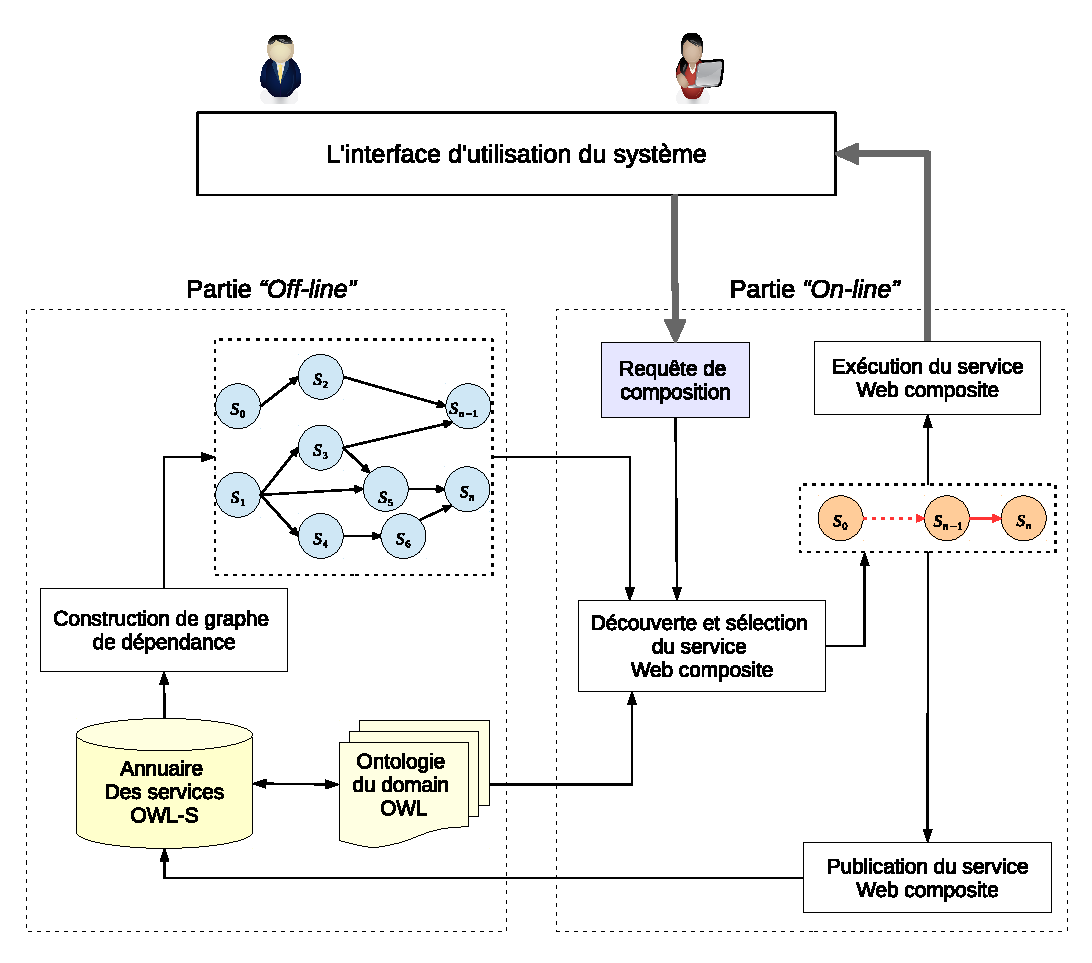
\includegraphics[width=1.15\textwidth]{figs/ch3/architecture.eps}
    \caption{Architecture générale du système.}
    \label{fig:ch3/architecture}
\end{figure}
%%% Local Variables:
%%% mode: latex
%%% TeX-master: "../../main"
%%% End:


L'architecture du système est articulé auteur de trois modules
principaux.
\subsubsection{Partie \emph{Off-line} du système}
\label{sec:presentation-architecture-online}

\subsubsection{Partie \emph{On-line} du système}
\label{sec:presentation-architecture-online}

\newpage
\section{Matching sémantique de services Web}
\label{sec:ch3/matching}

% Définition: Lien sémantique (ou dépendance fonctionnelle)%
% Définition: Matching Quality of a Link

\section{Construction du graphe de dépendance}
\label{sec:ch3/graph}

\section{Découverte de services Web composites}
\label{sec:ch3/composition}

\section*{Conclusion}
\label{sec:ch3/conclusion}
\addcontentsline{toc}{section}{Conclusion} \markboth{CONCLUSION}{}


%%% Local Variables:
%%% mode: latex
%%% TeX-master: "../main"
%%% End:
